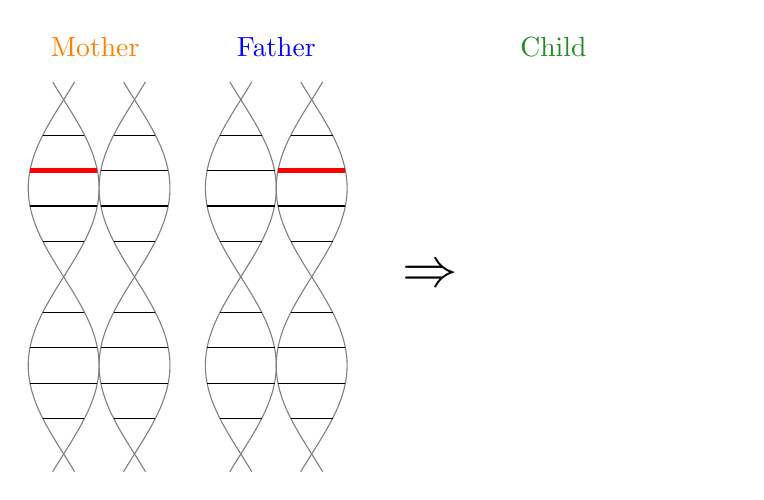
\begin{tikzpicture}
    % Draw the mother + father 
        \begin{scope}[scale=0.45, domain=-0.5:10.5, samples=110, rotate=90]
        %% Father
        \node[text width=1.0cm, color=blue] at (11.5, 0) {Father};
        %% Mother
        \node[text width=1.0cm, color=orange] at (11.5, 0 + 5.25) {Mother};
        % Draw the phosphate backbone, for each chromosome.
        \draw[gray] plot (\x,{sin(\x*36) + 1});
        \draw[gray] plot (\x,{-sin(\x*36) + 1});
        \draw[gray] plot (\x,{sin(\x*36) - 1});
        \draw[gray] plot (\x,{-sin(\x*36) - 1});
        % Draw the base pairs bonds
        \foreach \x in {0, 1, ..., 10}{
            \draw (\x, {-sin(\x*36) + 1}) -- (\x, {sin(\x*36) + 1});
            \draw (\x, {-sin(\x*36) - 1}) -- (\x, {sin(\x*36) - 1});
        }
        % Draw the phosphate backbone for mother
        \draw[gray] plot (\x, {sin(\x*36) + 4});
        \draw[gray] plot (\x, {-sin(\x*36) + 4});
        \draw[gray] plot (\x, {sin(\x*36) + 6});
        \draw[gray] plot (\x, {-sin(\x*36) + 6});
        % Draw the base pairs bonds
        \foreach \x in {0, 1, ..., 10}{
            \draw (\x, {-sin(\x*36) + 4}) -- (\x, {sin(\x*36) + 4});
            \draw (\x, {-sin(\x*36) + 6}) -- (\x, {sin(\x*36) + 6});
        }
        % Draw the one copy on each parent, at j = 8.
        \foreach \x in {8}{
            \draw[red, ultra thick] (\x, {-sin(\x*36) - 1}) -- (\x, {sin(\x*36) - 1});
            \draw[red, ultra thick] (\x, {-sin(\x*36) + 6}) -- (\x, {sin(\x*36) + 6});
        }
    %% Bridge to the child's genome
    \node[text width=2cm, scale=2] at (5, -8) {$\Rightarrow$};
    \node[text width=1.0cm, scale=1, color=ForestGreen] at (11.5, -8) {Child};
    \end{scope}
\end{tikzpicture}
